% Fig. 3 (input from main.tex): both faces, and both components joining the gluing loci C (delta = 1) and C' (delta = -1).
% Coordinates (x, depth, delta); the components bulge to depth -/+ b (1 - delta^2), front = F72^+, back = F72^-.
% The eight branches run from psi on C to the four real points of C' (up to diagonal local unitaries), one branch from
% each component to each point; the numbers are their classes (Theorem 1).  Dotted: path from the uniform state with
% four imaginary coefficients (in F72^+, delta = 0) to psi.
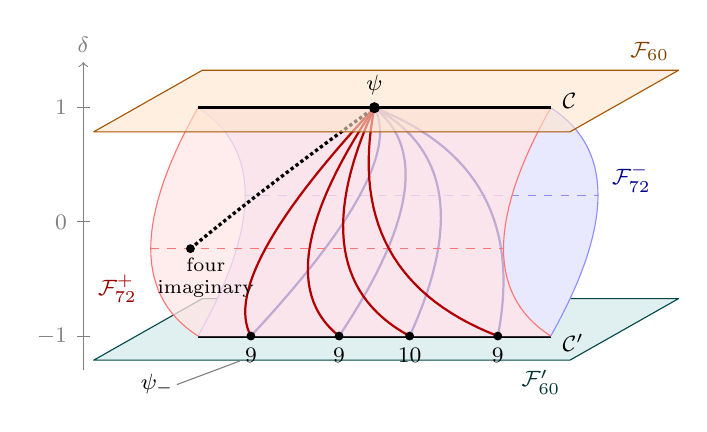
\begin{tikzpicture}[x={(0.56cm,0cm)},y={(0.30cm,0.17cm)},z={(0cm,1.45cm)},line join=round,font=\footnotesize]
  \def\b{2.0}
  \def\ends{1.2/9,3.2/9,4.8/10,6.8/9}
  % delta axis
  \draw[->,gray] (-2.6,0,-1.3) -- (-2.6,0,1.4) node[above] {$\delta$};
  \foreach \z in {1,0,-1} { \draw[gray] (-2.75,0,\z) -- (-2.45,0,\z) node[pos=0,left] {$\z$}; }
  % opposite face F60' and C'
  \fill[teal!12] (-1.4,-1.8,-1) -- (9.4,-1.8,-1) -- (9.4,2.8,-1) -- (-1.4,2.8,-1) -- cycle;
  \draw[teal!55!black] (-1.4,-1.8,-1) -- (9.4,-1.8,-1) -- (9.4,2.8,-1) -- (-1.4,2.8,-1) -- cycle;
  \node[teal!40!black,anchor=north east] at (9.4,-1.8,-1) {$\mathcal F_{60}'$};
  \draw[very thick] (0,0,-1) -- (8,0,-1);
  \node[anchor=west] at (8.05,0,-1.06) {$\mathcal C'$};
  % back component F72^-
  \fill[blue!9] plot[domain=1:-1,variable=\t,samples=31] (8,{\b*(1-\t*\t)},\t)
                -- plot[domain=-1:1,variable=\t,samples=31] (0,{\b*(1-\t*\t)},\t) -- cycle;
  \foreach \xx in {0,8} { \draw[blue!45] plot[domain=-1:1,variable=\t,samples=31] (\xx,{\b*(1-\t*\t)},\t); }
  \draw[blue!45,dashed] (0,\b,0) -- (8,\b,0);
  \foreach \e/\c in \ends { \draw[blue!60!black,thick] plot[domain=1:-1,variable=\t,samples=31]
                             ({4+(\e-4)*(1-\t)/2},{\b*(1-\t*\t)},\t); }
  \node[blue!55!black,anchor=west] at (8.1,\b,0.15) {$\mathcal F_{72}^-$};
  % front component F72^+
  \fill[red!10,opacity=0.75] plot[domain=1:-1,variable=\t,samples=31] (8,{-\b*(1-\t*\t)},\t)
                -- plot[domain=-1:1,variable=\t,samples=31] (0,{-\b*(1-\t*\t)},\t) -- cycle;
  \foreach \xx in {0,8} { \draw[red!55] plot[domain=-1:1,variable=\t,samples=31] (\xx,{-\b*(1-\t*\t)},\t); }
  \draw[red!55,dashed] (0,-\b,0) -- (8,-\b,0);
  \foreach \e/\c in \ends { \draw[red!70!black,thick] plot[domain=1:-1,variable=\t,samples=31]
                             ({4+(\e-4)*(1-\t)/2},{-\b*(1-\t*\t)},\t); }
  \node[red!60!black,anchor=east] at (-0.1,-\b,-0.35) {$\mathcal F_{72}^+$};
  % the uniform state with four imaginary coefficients and the path to psi
  \draw[densely dotted,very thick] plot[domain=0:0.97,variable=\t,samples=21] ({0.9+3.1*\t},{-\b*(1-\t*\t)},\t);
  \fill (0.9,-\b,0) circle (1.6pt);
  \node[anchor=north,align=center,font=\scriptsize,inner sep=1pt] at (1.25,-\b,-0.05) {four\\imaginary};
  % face F60 and C (drawn last: seen from above, it covers the top of the front component)
  \fill[orange!20,opacity=0.6] (-1.4,-1.8,1) -- (9.4,-1.8,1) -- (9.4,2.8,1) -- (-1.4,2.8,1) -- cycle;
  \draw[orange!65!black] (-1.4,-1.8,1) -- (9.4,-1.8,1) -- (9.4,2.8,1) -- (-1.4,2.8,1) -- cycle;
  \node[orange!50!black,anchor=south east] at (9.4,2.8,1) {$\mathcal F_{60}$};
  \draw[very thick] (0,0,1) -- (8,0,1);
  \node[anchor=west] at (8.05,0,1.06) {$\mathcal C$};
  % the real states
  \fill (4,0,1) circle (2pt) node[above=1pt] {$\ket\psi$};
  \foreach \e/\c in \ends { \fill (\e,0,-1) circle (1.6pt) node[below=1pt] {$\c$}; }
  \draw[gray] ([xshift=-4pt,yshift=-9pt]1.2,0,-1) -- ++(-0.8cm,-0.3cm) node[left,black,inner sep=1pt] {$\ket{\psi_-}$};
\end{tikzpicture}
